\chapter{Interfaces}\label{interfaces}


\section{Overview}\label{interfaces:overview}

The \texttt{interface} specification in a Dakota input file controls
details of function evaluations. The mechanisms currently in place for
function evaluations involve interfacing with one or more
computational simulation codes, computing algebraic mappings (refer to
Section~\ref{advint:algebraic}), or a combination of the two.

%In the case of use of an approximation in place of an expensive
%simulation code, an \texttt{approximation} interface can be selected
%to make use of surrogate modeling capabilities available within
%Dakota.  Surrogate models are discussed further in Chapter~\ref{models}.

This chapter will focus on mechanisms for simulation code invocation,
starting with interface types in Section~\ref{interfaces:sim} and
followed by a guide to constructing simulation-based interfaces in
Section~\ref{interfaces:building}.  This chapter also provides an
overview of simulation interface components, covers issues relating to
file management, and presents a number of example data mappings.

For a detailed description of interface specification syntax, refer to
the interface commands chapter in the Dakota Reference Manual~\cite{RefMan}.


\section{Simulation Interfaces}\label{interfaces:sim}

The invocation of a simulation code is performed using either system
calls or forks or via direct linkage. In the system call and fork
cases, a separate process is created for the simulation and
communication between Dakota and the simulation occurs through
parameter and response files. For system call and fork interfaces, the
interface section must specify the details of this data transfer.  In
the direct case, a separate process is not created and communication
occurs in memory through a prescribed API.
Sections~\ref{interfaces:direct} through \ref{interfaces:which}
provide information on the simulation interfacing approaches.

\subsection{Direct Simulation Interface}\label{interfaces:direct}

The direct interface may be used to invoke
simulations that are linked into the Dakota executable. This
interface eliminates overhead from process creation and file I/O and
can simplify operations on massively parallel computers. These
advantages are balanced with the practicality of converting an
existing simulation code into a library with a subroutine
interface. Sandia codes for structural dynamics (Salinas),
computational fluid dynamics (Sage), and circuit simulation (Xyce) and
external codes such as Phoenix Integration's ModelCenter framework and
The Mathworks' Matlab have been linked in this way, and a direct
interface to Sandia's SIERRA multiphysics framework is under
development. In the latter case, the additional effort is particularly
justified since SIERRA unifies an entire suite of physics codes.
[\emph{Note: the ``sandwich implementation'' of combining a direct
interface plug-in with Dakota's library mode is discussed in the
Dakota Developers Manual~\cite{DevMan}}].

In addition to direct linking with simulation codes, the direct
interface also provides access to internal polynomial test functions
that are used for algorithm performance and regression testing. The
following test functions are available: \texttt{cantilever},
\texttt{cyl\_head}, \texttt{log\_ratio}, \texttt{rosenbrock},
\texttt{short\_column}, and \texttt{text\_book} (including
\texttt{text\_book1}, \texttt{text\_book2}, \texttt{text\_book3}, and
\texttt{text\_book\_ouu}). While these functions are also available
as external programs in the \texttt{Dakota/test} directory,
maintaining internally linked versions allows more rapid testing. See
Chapter~\ref{additional} for additional information on several of
these test problems. An example input specification for a direct
interface follows:
\begin{small}
\begin{verbatim}
    interface,
            direct
              analysis_driver = 'rosenbrock'
\end{verbatim}
\end{small}

Additional specification examples are provided in
Section~\ref{tutorial:examples} and additional information on
asynchronous usage of the direct function interface is provided in
Section~\ref{parallel:SLP:local:direct}.  Guidance for usage of some
particular direct simulation interfaces is in
Section~\ref{advint:existingdirect} and the details of adding a
simulation code to the direct interface are provided in
Section~\ref{advint:direct}.

\subsection{System Call Simulation Interface}\label{interfaces:system}

{\bf Users are strongly encouraged to use the fork simulation
  interface if possible, though the system interface is still
  supported for portability and backward compatibility.}  The system
call approach invokes a simulation code or simulation driver by using
the \texttt{system} function from the standard C
library~\cite{Ker88}. In this approach, the system call creates a new
process that communicates with Dakota through parameter and response
files.  The system call approach allows the simulation to be initiated
via its standard invocation procedure (as a ``black box'') and then
coordinated with a variety of tools for pre- and post-processing.
This approach has been widely used in previous
studies~\cite{Eld96a,Eld96b,Eld98b}. The system call approach involves
more process creation and file I/O overhead than the direct function
approach, but this extra overhead is usually insignificant compared
with the cost of a simulation.  An example of a system call interface
specification follows:
\begin{small}
\begin{verbatim}
    interface,
            system
              analysis_driver = 'text_book'
              parameters_file = 'text_book.in'
              results_file    = 'text_book.out'
              file_tag file_save
\end{verbatim}
\end{small}

Information on asynchronous usage of the system interface is provided in
Section~\ref{parallel:SLP:local:system}.

\subsection{Fork Simulation Interface}\label{interfaces:fork}

The fork simulation interface uses the \texttt{fork}, \texttt{exec},
and \texttt{wait} families of functions to manage simulation codes or
simulation drivers. (In a native MS Windows version of Dakota, similar
Win32 functions, such as \texttt{\_spawnvp()}, are used instead.)
Calls to \texttt{fork} or \texttt{vfork} create a
copy of the Dakota process, \texttt{execvp} replaces this copy with
the simulation code or driver process, and then Dakota uses the
\texttt{wait} or \texttt{waitpid} functions to wait for completion of
the new process. Transfer of variables and response data between
Dakota and the simulator code or driver occurs through the file system
in exactly the same manner as for the system call interface. An
example of a fork interface specification follows:
\begin{small}
\begin{verbatim}
    interface,
            fork
              input_filter    = 'test_3pc_if'
              output_filter   = 'test_3pc_of'
              analysis_driver = 'test_3pc_ac'
              parameters_file = 'tb.in'
              results_file    = 'tb.out'
              file_tag
\end{verbatim}
\end{small}

More detailed examples of using the fork call interface are provided
in Section~\ref{tutorial:examples:user_supply:optimization1} and in
Section~\ref{interfaces:building}, and information on asynchronous usage
of the fork call interface is provided in
Section~\ref{parallel:SLP:local:fork}.


\subsection{Syntax for Filter and Driver Strings}\label{interfaces:syntax}

With the fork interface, and on most systems, with the system interface
as well, the string values supplied for \texttt{input\_filter}, \texttt{output\_filter},
and \texttt{analysis\_driver} can involve simple Bourne-shell
syntax for specifying environment values that the filter or driver will see.
For example,
\begin{verbatim}
    analysis_driver = 'opfile=myspec outlev=2 mydriver'
\end{verbatim}
would cause \texttt{mydriver} to be invoked with environment
variables \texttt{opfile} and \texttt{outlev} having the
values ``myspec" and ``2", respectively.  If the driver is a
shell script, it can access these values as \texttt{\$opfile} and
\texttt{\$outlev}; a compiled driver can obtain these values
from a function; drivers written in C or C++ can use the standard
\texttt{getenv} function (e.g., invoking \verb@getenv("opfile")@).

Both the values assigned to environment variables and name of the
file invoked as filter or driver can contain spaces, provided that the values
in question are quoted.  Within strings delimited by single quotes,
you can use double quotes for quoting, and vice versa.  For instance,
\begin{verbatim}
    analysis_driver = 'opfile="my spec" "my driver"'
\end{verbatim}
and
\begin{verbatim}
    analysis_driver = "opfile='my spec' 'my driver'"
\end{verbatim}
both specify a driver named ``\texttt{my driver}" and value ``\texttt{my spec}"
for \texttt{\$opfile}.



\subsection{Fork or System Call: Which to Use?}\label{interfaces:which}

The primary operational difference between the fork and system call
simulation interfaces is that, in the fork interface, the
\texttt{fork}/\texttt{exec} functions return a process identifier
that the \texttt{wait}/\texttt{waitpid} functions can use
to detect the completion of a simulation for either synchronous or
asynchronous operations.  The system call simulation interface, on the
other hand, must use a response file detection scheme for this purpose
in the asynchronous case. Thus, an important advantage of the fork
interface over the system call interface is that it avoids the
potential of a file race condition when employing asynchronous local
parallelism (refer to Section~\ref{parallel:SLP:local}). This condition
can occur when the responses file has been created but the writing of
the response data set to this file has not been completed (see
Section~\ref{parallel:SLP:local:system}). While significant care has been
taken to manage this file race condition in the system call case, the
fork interface still has the potential to be more robust when
performing function evaluations asynchronously.

Another advantage of the fork interface is that it has additional
asynchronous capabilities when a function evaluation involves multiple
analyses. As shown in Table~\ref{parallel:table01}, the fork interface
supports asynchronous local and hybrid parallelism modes for managing
concurrent analyses within function evaluations, whereas the system
call interface does not. These additional capabilities again stem from
the ability to track child processes by their process
identifiers.

The only disadvantage to the fork interface compared with
the system interface is that the
\texttt{fork}/\texttt{exec}/\texttt{wait} functions are not part of
the standard C library, whereas the \texttt{system} function is. As a
result, support for implementations of the
\texttt{fork}/\texttt{exec}/\texttt{wait} functions can vary from
platform to platform. At one time, these commands were not available
on some of Sandia's massively parallel computers. However, in the more
mainstream UNIX environments, availability of
\texttt{fork}/\texttt{exec}/\texttt{wait} should not be an issue.

In summary, the system call interface has been a workhorse for many
years and is well tested and proven, but the fork interface
supports additional capabilities and is recommended when managing
asynchronous simulation code executions. Having both interfaces
available has proven to be useful on a number of occasions and they
will both continue to be supported for the foreseeable future.


\section{Building a Black-Box Interface to a Simulation Code}\label{interfaces:building}

To interface a simulation code to Dakota using one of the black-box
interfaces (system call or fork), pre- and post-processing
functionality typically needs to be supplied (or developed) in order
to transfer the parameters from Dakota to the simulator input file and
to extract the response values of interest from the simulator's output
file for return to Dakota (see Figures~\ref{intro:bbinterface}
and~\ref{interfaces:bbinterfacecomp}). This is often managed through
the use of scripting languages, such as C-shell~\cite{And86}, Bourne
shell~\cite{Bli96}, Perl~\cite{Wal96}, or Python~\cite{Mar03}. While
these are common and convenient choices for simulation
drivers/filters, it is important to recognize that any executable file
can be used. If the user prefers, the desired pre- and post-processing
functionality may also be compiled or interpreted from any number of
programming languages (C, C++, F77, F95, JAVA, Basic, etc.).

In the \texttt{Dakota/examples/script\_interfaces/generic} directory,
a simple example uses the Rosenbrock test function as a mock
engineering simulation code. Several scripts have been included to
demonstrate ways to accomplish the pre- and post-processing
needs. Actual simulation codes will, of course, have different pre-
and post-processing requirements, and as such, this example serves
only to demonstrate the issues associated with interfacing a
simulator. Modifications will almost surely be required for new
applications.

\subsection{Generic Script Interface Files} 

The {\tt Dakota/examples/script\_interfaces/generic} directory contains four important files:
\texttt{dakota\_rosenbrock.in} (the Dakota input file),
\texttt{simulator\_script} (the simulation driver script),
\texttt{dprepro} (a pre-processing utility), and \\
\texttt{templatedir/ros.template} (a template simulation input file).

The file \texttt{dakota\_rosenbrock.in} specifies the study that
Dakota will perform and, in the interface section, describes the
components to be used in performing function evaluations. In
particular, it identifies \\ \texttt{simulator\_script} as its
\texttt{analysis\_driver}, as shown in Figure~\ref{advint:figure01}.
\begin{figure}
  \centering
  \begin{bigbox}
    \begin{small}
      \verbatimtabinput[8]{dakota_rosenbrock.in}
    \end{small}
  \end{bigbox}
  \caption{The \texttt{dakota\_rosenbrock.in} input file.}
  \label{advint:figure01}
\end{figure}

The \texttt{simulator\_script} listed in Figure~\ref{advint:figure02}
is a short driver shell script that Dakota executes to perform each
function evaluation. The names of the parameters and results files are
passed to the script on its command line; they are
referenced in the script by \texttt{\$argv[1]}
and \texttt{\$argv[2]}, respectively. The \texttt{simulator\_script}
is divided into three parts: pre-processing, analysis, and post-processing.
% is divided into five parts: set up, pre-processing, analysis,
% post-processing, and clean up.

\begin{figure}
  \centering
  \begin{bigbox}
    \begin{small}
      \verbatimtabinput[8]{simulator_script}
    \end{small}
  \end{bigbox}
  \caption{The \texttt{simulator\_script} sample driver script.}
  \label{advint:figure02}
\end{figure}

% The set up portion strips the function evaluation number from
% \texttt{\$argv[1]}and assigns it to the shell variable \texttt{\$num},
% which is then used to create a tagged working directory for a
% particular evaluation. For example, on the first evaluation,
% ``\texttt{1}'' is stripped from ``\texttt{params.in.1}'' in order to
% create ``\texttt{workdir.1}''. The primary reason for creating
% separate working directories is so that the files associated with one
% simulation do not conflict with those for another simulation. This is
% particularly important when executing concurrent simulations in
% parallel (to actually execute function evaluations concurrently,
% uncomment the \texttt{asynchronous} line in \texttt{dakota\_rosenbrock.in}).
% %Once executing within the confines of the working directory, tags on the 
% %files are no longer necessary, and for this reason, the tagged parameters
% %file is moved to a more convenient name of ``\texttt{dakota\_vars}''.

In the pre-processing portion, the \texttt{simulator\_script} uses
\texttt{dprepro}, a parsing utility, to extract the
current variable values from a parameters file (\texttt{\$argv[1]})
and combine them with the simulator template input file
(\texttt{ros.template}) to create a new input file (\texttt{ros.in})
for the simulator. Internal to Sandia, the APREPRO utility is often
used for this purpose. For external sites where APREPRO is not
available, the DPrePro utility mentioned above is an alternative with
many of the capabilities of APREPRO that is specifically tailored for
use with Dakota and is distributed with it (in
\\ \texttt{Dakota/examples/script\_interfaces/generic/dprepro}, or {\tt
Dakota/bin} in a binary distribution). Additionally, the BPREPRO
utility is another alternative to APREPRO (see~\cite{WalXX}), and at
Lockheed Martin sites, the JPrePost utility is available as a JAVA
pre- and post-processor~\cite{Fla}. The \texttt{dprepro} script
(usage shown in Figure~\ref{advint:figure03}) will be used here for
simplicity of discussion. It can use either Dakota's \texttt{aprepro}
parameters file format (see
Section~\ref{variables:parameters:aprepro}) or Dakota's standard
format (see Section~\ref{variables:parameters:standard}), so either
option may be selected in the interface section of the Dakota input
file. The \texttt{ros.template} file listed in
Figure~\ref{advint:figure04} is a template simulation input file which
contains targets for the incoming variable values, identified by the
strings ``\texttt{\{x1\}}'' and ``\texttt{\{x2\}}''. These
identifiers match the variable descriptors specified in
\texttt{dakota\_rosenbrock.in}. The template input file is contrived
as Rosenbrock has nothing to do with finite element analysis; it only
mimics a finite element code to demonstrate the simulator
template process. The \texttt{dprepro} script will search the
simulator template input file for fields marked with curly
brackets and then create a new file (\texttt{ros.in}) by replacing
these targets with the corresponding numerical values for the
variables. As noted in the usage information for \texttt{dprepro} and
shown in \texttt{simulator\_script}, the names for the Dakota
parameters file (\texttt{\$argv[1]}), template file
(\texttt{ros.template}), and generated input file (\texttt{ros.in})
must be specified in the \texttt{dprepro} command line arguments.

\begin{figure}
  \centering
  \begin{bigbox}
    \begin{small}
      \verbatimtabinput[8]{dprepro_usage}
    \end{small}
  \end{bigbox}
  \caption{Partial listing of the \texttt{dprepro} script.}
  \label{advint:figure03}
\end{figure}

\begin{figure}
  \centering
  \begin{bigbox}
    \begin{small}
      \verbatimtabinput[8]{ros.template}
    \end{small}
  \end{bigbox}
  \caption{Listing of the \texttt{ros.template} file}
  \label{advint:figure04}
\end{figure}

The second part of the script executes the \texttt{rosenbrock\_bb}
simulator. The input and output file names, \texttt{ros.in} and
\texttt{ros.out}, respectively, are hard-coded into the FORTRAN 77
program \texttt{rosenbrock\_bb.f}. When the \texttt{rosenbrock\_bb}
simulator is executed, the values for \texttt{x1} and \texttt{x2} are
read in from \texttt{ros.in}, the Rosenbrock function is evaluated,
and the function value is written out to \texttt{ros.out}.

The third part performs the post-processing and writes the response
results to a file for Dakota to read. Using the UNIX ``\texttt{grep}'' utility, the
particular response values of interest are extracted from the raw
simulator output and saved to a temporary file (\texttt{results.tmp}).
When complete, this file is renamed \texttt{\$argv[2]}, which in this
example is always ``\texttt{results.out}''.
Note that moving or renaming the completed results file
avoids any problems with read race
conditions (see Section~\ref{parallel:SLP:local:system}).

% Finally, in the clean up phase, the working directory is removed to
% reduce the amount of disk storage required to execute the study. If
% data from each simulation needs to be saved, this step can be
% commented out by inserting a ``\texttt{\#}'' character before
% ``\texttt{$\backslash$rm -rf}''.

Because the Dakota input file \texttt{dakota\_rosenbrock.in}
(Figure~\ref{advint:figure01}) specifies
\texttt{work\_directory} and \texttt{directory\_tag} in its interface
section, each invocation of \texttt{simulator\_script} wakes up in
its own temporary directory, which Dakota has populated with the
contents of directory \texttt{templatedir}. Having a separate directory
for each invocation of \texttt{simulator\_script} simplifies the script
when the Dakota input file specifies \texttt{asynchronous} (so
several instances of \texttt{simulator\_script} might run simultaneously),
as fixed names such as \texttt{ros.in}, \texttt{ros.out}, and \texttt{results.tmp}
can be used for intermediate files. If neither \texttt{asynchronous} nor
\texttt{file\_tag} is specified, and if there is no need (e.g., for debugging)
to retain intermediate files having fixed names, then \texttt{directory\_tag}
offers no benefit and can be omitted. An alternative to \texttt{directory\_tag}
is to proceed as earlier versions of this chapter --- prior to Dakota 5.0's
introduction of \texttt{work\_directory} --- recommended:  add two more
steps to the \texttt{simulator\_script},
an initial one to create a temporary directory explicitly and
copy \texttt{templatedir} to it if needed, and a final step to remove the temporary
directory and any files in it.

When \texttt{work\_directory} is specified, Dakota adjusts the \texttt{\$PATH} seen
by \texttt{simulator\_script} so that simple program names
%in the \texttt{simulator\_script}
(i.e., names not containing a slash) that
are visible in Dakota's directory will also be visible in the work directory.
Relative path names ---
involving an intermediate slash but not an initial one,
such as \texttt{./rosenbrock\_bb} or \texttt{a/bc/rosenbrock\_bb} ---
will only be visible in the work directory if a \texttt{link\_files}
or \texttt{copy\_files} specification (see \S\ref{interfaces:workdir})
has made them visible there.

As an example of the data flow on a particular function evaluation,
consider evaluation 60. The parameters file for this evaluation consists of:
\begin{small}
\begin{verbatim}
    { DAKOTA_VARS     =                      2 }
    { x1              =  1.638247697999295e-01 }
    { x2              =  2.197298209103481e-02 }
    { DAKOTA_FNS      =                      1 }
    { ASV_1           =                      1 }
    { DAKOTA_DER_VARS =                      2 }
    { DVV_1           =                      1 }
    { DVV_2           =                      2 }
    { DAKOTA_AN_COMPS =                      0 }
\end{verbatim}
\end{small}

This file is called \texttt{workdir/workdir.60/params.in} if the line
\begin{small}
\begin{verbatim}
 	  named 'workdir' file_save  directory_save
\end{verbatim}
\end{small}
in Figure~\ref{advint:figure01} is uncommented.
The first portion of the file indicates that there are two variables,
followed by new values for variables \texttt{x1} and \texttt{x2}, and
one response function (an objective function), followed by an active
set vector (ASV) value of \texttt{1}. The ASV indicates the need to
return the value of the objective function for these parameters (see
Section~\ref{variables:asv}). The \texttt{dprepro} script reads the
variable values from this file, namely \texttt{1.638247697999295e-01}
and \texttt{2.197298209103481e-02} for \texttt{x1} and \texttt{x2}
respectively, and substitutes them in the \texttt{\{x1\}} and
\texttt{\{x2\}} fields of the \texttt{ros.template} file. The final
three lines of the resulting input file (\texttt{ros.in}) then appear
as follows:
\begin{small}
\begin{verbatim}
    variable 1 1.638247697999295e-01
    variable 2 2.197298209103481e-02
    end
\end{verbatim}
\end{small}

where all other lines are identical to the template file. The
\texttt{rosenbrock\_bb} simulator accepts \texttt{ros.in} as its input
file and generates the following output to the file \texttt{ros.out}:
\begin{small}
\begin{verbatim}
    Beginning execution of model: Rosenbrock black box
    Set up complete.
    Reading nodes.
    Reading elements.
    Reading materials.
    Checking connectivity...OK
    *****************************************************

    Input value for x1 =  0.1638247697999295E+00
    Input value for x2 =  0.2197298209103481E-01

    Computing solution...Done
    *****************************************************
    Function value =  0.7015563957680092E+00
    Function gradient = [ -0.1353509902591768E+01 -0.9731146217930163E+00 ]
\end{verbatim}
\end{small}

Next, the appropriate values are extracted from the raw simulator output
and returned in the results file. This post-processing is relatively
trivial in this case, and the \texttt{simulator\_script} uses the
\texttt{grep} and \texttt{cut} utilities to extract the value from the
``\texttt{Function value}" line of the \texttt{ros.out} output file and save it to
\texttt{\$argv[2]}, which is the \texttt{results.out} file for this
evaluation. This single value provides the objective function value
requested by the ASV.

After 132 of these function evaluations, the following Dakota output
shows the final solution using the \\ \texttt{rosenbrock\_bb} simulator:
\begin{small}
\begin{verbatim}
    Exit NPSOL - Optimal solution found.

    Final nonlinear objective value =   0.1165704E-06

   NPSOL exits with INFORM code = 0 (see "Interpretation of output" section in NPSOL manual)

   NOTE: see Fortran device 9 file (fort.9 or ftn09)
         for complete NPSOL iteration history.

   <<<<< Iterator npsol_sqp completed.
   <<<<< Function evaluation summary: 132 total (132 new, 0 duplicate)
   <<<<< Best parameters          =
                         9.9965861667e-01 x1
                         9.9931682203e-01 x2
   <<<<< Best objective function  =
                      1.1657044253e-07
   <<<<< Best data captured at function evaluation 130

   <<<<< Iterator npsol_sqp completed.
   <<<<< Single Method Strategy completed.
   Dakota execution time in seconds:
     Total CPU        =       0.12 [parent =   0.116982, child =   0.003018]
     Total wall clock =    1.47497
\end{verbatim}
\end{small}

\subsection{Adapting These Scripts to Another Simulation}

To adapt this approach for use with another simulator, several steps
need to be performed:

\begin{enumerate}
\item Create a template simulation input file by identifying the fields
  in an existing input file that correspond to the variables of
  interest and then replacing them with \texttt{\{\}} identifiers
  (e.g. \texttt{\{cdv\_1\}}, \texttt{\{cdv\_2\}}, etc.) which match
  the Dakota variable descriptors. Copy this template input file to a
  templatedir that will be used to create working directories for the
  simulation.

\item Modify the \texttt{dprepro} arguments in
  \texttt{simulator\_script} to reflect names of the Dakota parameters
  file (previously ``\texttt{\$argv[1]}''), template file name
  (previously ``\texttt{ros.template}'') and generated input file
  (previously ``\texttt{ros.in}''). Alternatively, use APREPRO,
  BPREPRO, or JPrePost to perform this step (and adapt the syntax
  accordingly).

\item Modify the analysis section of \texttt{simulator\_script} to
  replace the \texttt{rosenbrock\_bb} function call with the new
  simulator name and command line syntax (typically including the
  input and output file names).

\item Change the post-processing section in \texttt{simulator\_script}
  to reflect the revised extraction process. At a minimum, this would
  involve changing the \texttt{grep} command to reflect the name of
  the output file, the string to search for, and the characters to cut
  out of the captured output line. For more involved post-processing
  tasks, invocation of additional tools may have to be added to the
  script.

\item Modify the \texttt{dakota\_rosenbrock.in} input file to reflect,
  at a minimum, updated variables and responses specifications.
\end{enumerate}

These nonintrusive interfacing approaches can be used to rapidly
interface with simulation codes. While generally custom for each new
application, typical interface development time is on the order of an
hour or two. Thus, this approach is scalable when dealing with many
different application codes. Weaknesses of this approach include the
potential for loss of data precision (if care is not taken to preserve
precision in pre- and post-processing file I/O), a lack of robustness
in post-processing (if the data capture is too simplistic), and
scripting overhead (only noticeable if the simulation time is on the
order of a second or less).

If the application scope at a particular site is more focused and only
a small number of simulation codes are of interest, then more
sophisticated interfaces may be warranted. For example, the economy of
scale afforded by a common simulation framework justifies additional
effort in the development of a high quality Dakota interface. In these
cases, more sophisticated interfacing approaches could involve a more
thoroughly developed black box interface with robust support of a
variety of inputs and outputs, or it might involve intrusive
interfaces such as the direct simulation interface discussed below in
Section~\ref{advint:direct} or the SAND interface described in
Section~\ref{intro:coupling}.

\subsection{Additional Examples}

A variety of additional examples of black-box interfaces to simulation
codes are maintained in the\\
\texttt{Dakota/examples/script\_interfaces} directory in the source
code distribution.


\section{Simulation Interface Components}\label{interfaces:components}


Figure~\ref{interfaces:bbinterfacecomp} is an extension of
Figure~\ref{intro:bbinterface} that adds details of the
components that make up each of the simulation interfaces (system
call, fork, and direct).  These components include an
\texttt{input\_filter} (``IFilter''), one or more
\texttt{analysis\_drivers} (``Analysis Code/Driver''), and an
\texttt{output\_filter} (``OFilter''). The input and output filters
provide optional facilities for managing simulation pre- and
post-processing, respectively. More specifically, the input filter can
be used to insert the Dakota parameters into the input files required
by the simulator program, and the output filter can be used to recover
the raw data from the simulation results and compute the desired
response data set. If there is a single analysis code, it is often
convenient to combine these pre- and post-processing functions into a
single simulation driver script, and the separate input and output
filter facilities are rarely used in this case. If there are multiple
analysis drivers, however, the input and output filter facilities
provide a convenient means for managing \emph{non-repeated} portions of
the pre- and post-processing for multiple analyses. That is, pre- and
post-processing tasks that must be performed for each analysis can be
performed within the individual analysis drivers, and shared pre- and
post-processing tasks that are only performed once for the set of
analyses can be performed within the input and output filters.

\begin{figure}
  \centering
  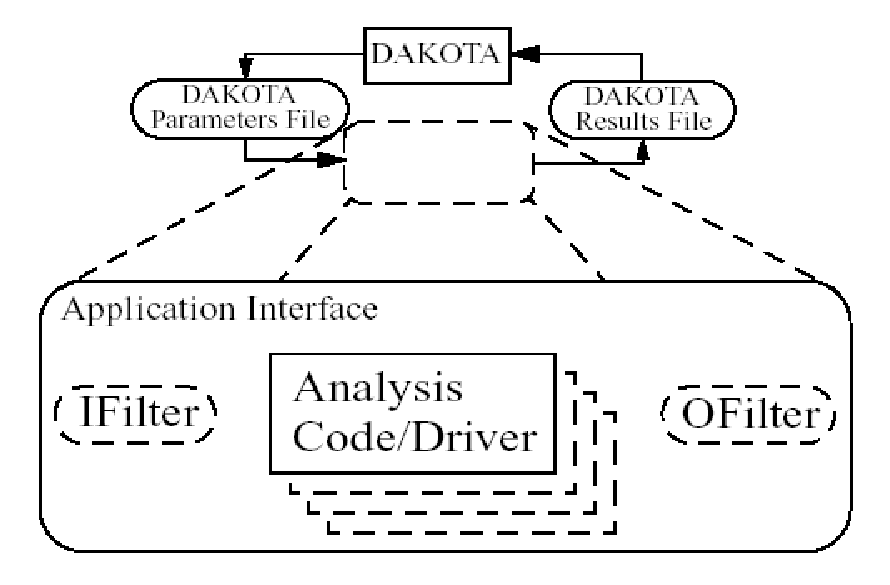
\includegraphics[scale=0.8]{images/dakota_components}
  \caption{Components of the simulation interface}
  \label{interfaces:bbinterfacecomp}
\end{figure}

When spawning function evaluations using system calls or forks, Dakota
must communicate parameter and response data with the analysis drivers
and filters through use of the file system. This is accomplished by
passing the names of the parameters and results files on the command
line when executing an analysis driver or filter. The input filter or
analysis driver read data from the parameters file and the output
filter or analysis driver write the appropriate data to the responses
file. While not essential when the file names are fixed, the file
names must be retrieved from the command line when Dakota is changing
the file names from one function evaluation to the next (i.e., using
temporary files or root names tagged with numerical identifiers).
In the case of a UNIX C-shell script, the two command line arguments
are retrieved using \texttt{\$argv[1]} and \texttt{\$argv[2]}
(see~\cite{And86}).  Similarly, Bourne shell scripts retrieve the two
command line arguments using \texttt{\$1} and \texttt{\$2}, and Perl
scripts retrieve the two command line arguments using
\texttt{@ARGV[0]} and \texttt{@ARGV[1]}.  In the case of a C or C++
program, command line arguments are retrieved using \texttt{argc}
(argument count) and \texttt{argv} (argument vector)~\cite{Ker88}, and
for Fortran 77, the \texttt{iargc} function returns the argument count
and the \texttt{getarg} subroutine returns command line arguments.

\subsection{Single analysis driver without filters}\label{interfaces:components:single1}

If a single \texttt{analysis\_driver} is selected in the interface
specification and filters are not needed (as indicated by omission of
the \texttt{input\_filter} and \texttt{output\_filter}
specifications), then only one process will appear in the execution
syntax of the simulation interface. An example of this syntax in the
system call case is:
\begin{small}
\begin{verbatim}
    driver params.in results.out
\end{verbatim}
\end{small}

where ``\texttt{driver}'' is the user-specified analysis driver and
``\texttt{params.in}'' and ``\texttt{results.out}'' are the names of the
parameters and results files, respectively, passed on the command
line. In this case, the user need not retrieve the command line
arguments since the same file names will be used each time.

For the same mapping, the fork simulation interface echoes the
following syntax:
\begin{small}
\begin{verbatim}
    blocking fork: driver params.in results.out
\end{verbatim}
\end{small}

for which only a single blocking fork is needed to perform the
evaluation.

Executing the same mapping with the direct simulation interface
results in an echo of the following syntax:
\begin{small}
\begin{verbatim}
    Direct function: invoking driver
\end{verbatim}
\end{small}

where this analysis driver must be linked as a function within
Dakota's direct interface (see Section~\ref{advint:direct}). Note that
no parameter or response files are involved, since such values
are passed directly through the function argument lists.

Both the system call and fork interfaces support asynchronous
operations. The asynchronous system call execution syntax involves
executing the system call in the background:
\begin{small}
\begin{verbatim}
    driver params.in.1 results.out.1 &
\end{verbatim}
\end{small}

and the asynchronous fork execution syntax involves use of a
nonblocking fork:
\begin{small}
\begin{verbatim}
    nonblocking fork: driver params.in.1 results.out.1
\end{verbatim}
\end{small}

where file tagging (see Section~\ref{interfaces:file:tagging1}) has
been user-specified in both cases to prevent conflicts between
concurrent analysis drivers. In these cases, the user must retrieve
the command line arguments since the file names change on each
evaluation.  Execution of the direct interface must currently be
performed synchronously since multithreading is not yet supported
(see Section~\ref{parallel:SLP:local:direct}).

\subsection{Single analysis driver with filters}\label{interfaces:components:single2}

When filters are used, the syntax of the system call that Dakota
performs is:
\begin{small}
\begin{verbatim}
    ifilter params.in results.out; driver params.in results.out;
         ofilter params.in results.out
\end{verbatim}
\end{small}

in which the input filter (``\texttt{ifilter}''), analysis driver
(``\texttt{driver}''), and output filter (``\texttt{ofilter}'')
processes are combined into a single system call through the use of
semi-colons (see~\cite{And86}). All three portions are
passed the names of the parameters and results files on the command
line.

For the same mapping, the fork simulation interface echoes the
following syntax:
\begin{small}
\begin{verbatim}
    blocking fork: ifilter params.in results.out;
         driver params.in results.out; ofilter params.in results.out
\end{verbatim}
\end{small}

where a series of three blocking forks is used to perform the
evaluation.

Executing the same mapping with the direct simulation interface
results in an echo of the following syntax:
\begin{small}
\begin{verbatim}
    Direct function: invoking { ifilter driver ofilter }
\end{verbatim}
\end{small}

where each of the three components must be linked as a function within
Dakota's direct interface. Since asynchronous operations are not yet
supported, execution simply involves invocation of each of the three
linked functions in succession. Again, no files are involved since
parameter and response data are passed directly through the function
argument lists.

Asynchronous executions would appear as follows for the system call
interface:
\begin{small}
\begin{verbatim}
    (ifilter params.in.1 results.out.1; driver params.in.1 results.out.1;
         ofilter params.in.1 results.out.1) &
\end{verbatim}
\end{small}

and, for the fork interface, as:
\begin{small}
\begin{verbatim}
    nonblocking fork: ifilter params.in.1 results.out.1;
         driver params.in.1 results.out.1; ofilter params.in.1 results.out.1
\end{verbatim}
\end{small}

where file tagging of evaluations has again been user-specified in
both cases. For the system call simulation interface, use of
parentheses and semi-colons to bind the three processes into a single
system call simplifies asynchronous process management compared to an
approach using separate system calls. The fork simulation interface,
on the other hand, does not rely on parentheses and accomplishes
asynchronous operations by first forking an intermediate process. This
intermediate process is then reforked for the execution of the input
filter, analysis driver, and output filter. The intermediate process
can be blocking or nonblocking (nonblocking in this case), and the
second level of forks can be blocking or nonblocking (blocking in this
case). The fact that forks can be reforked multiple times using either
blocking or nonblocking approaches provides the enhanced flexibility
to support a variety of local parallelism approaches (see
Chapter~\ref{parallel}).

\subsection{Multiple analysis drivers without filters}\label{interfaces:components:multiple1}

If a list of \texttt{analysis\_drivers} is specified and filters are
not needed (i.e., neither \texttt{input\_filter} nor
\texttt{output\_filter} appears), then the system call syntax
would appear as:
\begin{small}
\begin{verbatim}
    driver1 params.in results.out.1; driver2 params.in results.out.2;
         driver3 params.in results.out.3
\end{verbatim}
\end{small}

where ``\texttt{driver1}'', ``\texttt{driver2}'', and
``\texttt{driver3}'' are the user-specified analysis drivers and
``\texttt{params.in}'' and ``\texttt{results.out}'' are the
user-selected names of the parameters and results files. Note that the
results files for the different analysis drivers have been
automatically tagged to prevent overwriting. This automatic tagging of
\emph{analyses} (see Section~\ref{interfaces:file:tagging2}) is a
separate operation from user-selected tagging of \emph{evaluations}
(see Section~\ref{interfaces:file:tagging1}).

For the same mapping, the fork simulation interface echoes the
following syntax:
\begin{small}
\begin{verbatim}
    blocking fork: driver1 params.in results.out.1;
         driver2 params.in results.out.2; driver3 params.in results.out.3
\end{verbatim}
\end{small}

for which a series of three blocking forks is needed (no reforking of
an intermediate process is required).

Executing the same mapping with the direct simulation interface
results in an echo of the following syntax:
\begin{small}
\begin{verbatim}
    Direct function: invoking { driver1 driver2 driver3 }
\end{verbatim}
\end{small}

where, again, each of these components must be linked within Dakota's
direct interface and no files are involved for parameter and response
data transfer.

Both the system call and fork interfaces support asynchronous function
evaluations. The asynchronous system call execution syntax would be
reported as
\begin{small}
\begin{verbatim}
    (driver1 params.in.1 results.out.1.1; driver2 params.in.1 results.out.1.2;
         driver3 params.in.1 results.out.1.3) &
\end{verbatim}
\end{small}

and the nonblocking fork execution syntax would be reported as
\begin{small}
\begin{verbatim}
    nonblocking fork: driver1 params.in.1 results.out.1.1;
         driver2 params.in.1 results.out.1.2; driver3 params.in.1 results.out.1.3
\end{verbatim}
\end{small}

where, in both cases, file tagging of evaluations has been
user-specified to prevent conflicts between concurrent analysis
drivers and file tagging of the results files for multiple analyses is
automatically used. In the fork interface case, an intermediate
process is forked to allow a non-blocking function evaluation, and
this intermediate process is then reforked for the execution of each
of the analysis drivers.

\subsection{Multiple analysis drivers with filters}\label{interfaces:components:multiple2}

Finally, when combining filters with multiple
\texttt{analysis\_drivers}, the syntax of the system call that Dakota
performs is:
\begin{small}
\begin{verbatim}
    ifilter params.in.1 results.out.1;
         driver1 params.in.1 results.out.1.1;
         driver2 params.in.1 results.out.1.2;
         driver3 params.in.1 results.out.1.3;
         ofilter params.in.1 results.out.1
\end{verbatim}
\end{small}

in which all processes have again been combined into a single system
call through the use of semi-colons and parentheses. Note that the
secondary file tagging for the results files is only used for the
analysis drivers and not for the filters. This is consistent with the
filters' defined purpose of managing the non-repeated portions of
analysis pre- and post-processing (e.g., overlay of response results
from individual analyses; see Section~\ref{interfaces:file:tagging2}
for additional information).

For the same mapping, the fork simulation interface echoes the
following syntax:
\begin{small}
\begin{verbatim}
    blocking fork: ifilter params.in.1 results.out.1;
         driver1 params.in.1 results.out.1.1;
         driver2 params.in.1 results.out.1.2;
         driver3 params.in.1 results.out.1.3;
         ofilter params.in.1 results.out.1
\end{verbatim}
\end{small}

for which a series of five blocking forks is used (no reforking of an
intermediate process is required).

Executing the same mapping with the direct simulation interface
results in an echo of the following syntax:
\begin{small}
\begin{verbatim}
    Direct function: invoking { ifilter driver1 driver2 driver3 ofilter }
\end{verbatim}
\end{small}

where each of these components must be linked as a function within
Dakota's direct interface. Since asynchronous operations are not
supported, execution simply involves invocation of each of the five
linked functions in succession. Again, no files are involved for
parameter and response data transfer since this data is passed
directly through the function argument lists.

Asynchronous executions would appear as follows for the system call
interface:
\begin{small}
\begin{verbatim}
    (ifilter params.in.1 results.out.1;
         driver1 params.in.1 results.out.1.1;
         driver2 params.in.1 results.out.1.2;
         driver3 params.in.1 results.out.1.3;
         ofilter params.in.1 results.out.1) &
\end{verbatim}
\end{small}

and for the fork interface:
\begin{small}
\begin{verbatim}
    nonblocking fork: ifilter params.in.1 results.out.1;
         driver1 params.in.1 results.out.1.1;
         driver2 params.in.1 results.out.1.2;
         driver3 params.in.1 results.out.1.3;
         ofilter params.in.1 results.out.1
\end{verbatim}
\end{small}

where, again, user-selected file tagging of evaluations is combined
with automatic file tagging of analyses. In the fork interface case,
an intermediate process is forked to allow a non-blocking function
evaluation, and this intermediate process is then reforked for the
execution of the input filter, each of the analysis drivers, and the
output filter.

A complete example of these filters and multi-part drivers can be
found in \texttt{Dakota/test/dakota\_3pc/dakota\_3pc.in}.

\section{Simulation File Management}\label{interfaces:file}

This section describes some management features used for files that
transfer data between Dakota and simulation codes
(i.e., when the system call or fork interfaces are used). These
features can generate unique filenames when
Dakota executes programs in parallel and can help one debug
the interface between Dakota and a simulation code.

\subsection{File Saving}\label{interfaces:file:saving}

{\bf Before driver execution:} In Dakota 5.0 and newer, an existing
results file will be removed immediately prior to executing the
analysis driver.  This new behavior addresses a common user problem
resulting from starting Dakota with stale results files in the run
directory.  To override this default behavior and preserve any
existing results files, specify \texttt{allow\_existing\_results}.

{\bf After driver execution:} The \texttt{file\_save} option in the
interface specification allows the user to control whether parameters
and results files are retained or removed from the working directory
after the analysis completes. Dakota's default behavior is to remove
files once their use is complete to reduce clutter. If the method
output setting is verbose, a file remove notification will follow the
function evaluation echo, e.g.,
\begin{small}
\begin{verbatim}
    driver /usr/tmp/aaaa20305 /usr/tmp/baaa20305
    Removing /usr/tmp/aaaa20305 and /usr/tmp/baaa20305
\end{verbatim}
\end{small}

However, if \texttt{file\_save} appears in the interface
specification, these files will not be removed. This latter behavior
is often useful for debugging communication between Dakota and
simulator programs. An example of a \texttt{file\_save} specification
is shown in the file tagging example below.

\subsection{File Tagging for Evaluations}\label{interfaces:file:tagging1}

When a user provides \texttt{parameters\_file} and
\texttt{results\_file} specifications, the \texttt{file\_tag} option
in the interface specification causes Dakota to make the names of
these files unique by appending the function
evaluation number to the root file names. Default behavior is to not
tag these files, which has the advantage of allowing the user to
ignore command line argument passing and always read to and write from
the same file names. However, it has the disadvantage that files may
be overwritten from one function evaluation to the next. When
\texttt{file\_tag} appears in the interface specification, the file names
are made unique by the appended evaluation number. This uniqueness
requires the user's interface to get the names of
these files from the command line. The file tagging feature is most
often used when concurrent simulations are running in a common disk
space, since it can prevent conflicts between the simulations. An
example specification of \texttt{file\_tag} and \texttt{file\_save} is
shown below:
\begin{small}
\begin{verbatim}
    interface,
            system
              analysis_driver = 'text_book'
              parameters_file = 'text_book.in'
              results_file    = 'text_book.out'
              file_tag file_save
\end{verbatim}
\end{small}

\emph{Special case:} When a user specifies names for the parameters
and results files and \texttt{file\_save} is used without
\texttt{file\_tag}, untagged files are used in the function evaluation
but are then moved to tagged files after the function evaluation is
complete, to prevent overwriting files for which a
\texttt{file\_save} request has been given. If the output control is
set to verbose, then a notification similar to the following will
follow the function evaluation echo:
\begin{small}
\begin{verbatim}
    driver params.in results.out
    Files with non-unique names will be tagged to enable file_save:
    Moving params.in to params.in.1
    Moving results.out to results.out.1
\end{verbatim}
\end{small}

\textbf{Hierarchical tagging:} When a model's specification includes
the {\tt hierarchical\_tagging} keyword, the tag applied to parameter
and results file names of any subordinate interfaces will reflect any
model hierarchy present.  This option is useful for studies involving
multiple models with a nested or hierarchical relationship.  For
example a nested model has a sub-method, which itself likely operates
on a sub-model, or a hierarchical approximation involves coordination
of low and high fidelity models.  Specifying {\tt
  hierarchical\_tagging} will yield function evaluation identifiers
(``tags'') composed of the evaluation IDs of the models involved,
e.g., outermodel.innermodel.interfaceid = 4.9.2.  This communicates
the outer contexts to the analysis driver when performing a function
evaluation.  For an example of using hierarhical tagging in a nested
model context, see {\tt
  dakota/test/dakota\_uq\_timeseries\_*\_optinterf.in}.

\subsection{Temporary Files}\label{interfaces:file:temporary}

If \texttt{parameters\_file} and \texttt{results\_file} are not
specified by the user, temporary files having generated names are
used.  For example, a system call to a single analysis driver might
appear as:
\begin{small}
\begin{verbatim}
    driver /tmp/dakota_params_aaaa2035 /tmp/dakota_results_baaa2030
\end{verbatim}
\end{small}

and a system call to an analysis driver with filter programs might appear as:
\begin{small}
\begin{verbatim}
    ifilter /tmp/dakota_params_aaaa2490 /tmp/dakota_results_baaa2490;
         driver /tmp/dakota_params_aaaa2490 tmp/dakota_results_baaa2490;
         ofilter /tmp/dakota_params_aaaa2490 /tmp/dakota_results_baa22490
\end{verbatim}
\end{small}

These files have unique names created by Boost filesystem
utilities. This uniqueness requires the user's interface to get the
names of these files from the command line. File tagging with
evaluation number is unnecessary with temporary files, but can be
helpful for the user workflow to identify the evaluation number.  Thus
\texttt{file\_tag} requests will be honored. A \texttt{file\_save}
request will be honored, but it should be used with care since the
temporary file directory could easily become cluttered without the
user noticing.

\subsection{File Tagging for Analysis Drivers}\label{interfaces:file:tagging2}

When multiple analysis drivers are involved in performing a function
evaluation with either the system call or fork simulation interface,
a secondary file tagging is \emph{automatically} used to
distinguish the results files used for the individual analyses. This
applies to both the case of user-specified names for the parameters
and results files and the default temporary file case. Examples
for the former case were shown previously in
Section~\ref{interfaces:components:multiple1} and
Section~\ref{interfaces:components:multiple2}.  The following examples
demonstrate the latter temporary file case. Even though Unix
temporary files have unique names for a particular function
evaluation, tagging is still needed to manage the individual
contributions of the different analysis drivers to the response
results, since the same root results filename is used for each
component. For the system call interface, the syntax would be similar
to the following:
\begin{small}
\begin{verbatim}
    ifilter /var/tmp/aaawkaOKZ /var/tmp/baaxkaOKZ;
         driver1 /var/tmp/aaawkaOKZ /var/tmp/baaxkaOKZ.1;
         driver2 /var/tmp/aaawkaOKZ /var/tmp/baaxkaOKZ.2;
         driver3 /var/tmp/aaawkaOKZ /var/tmp/baaxkaOKZ.3;
         ofilter /var/tmp/aaawkaOKZ /var/tmp/baaxkaOKZ
\end{verbatim}
\end{small}

and, for the fork interface, similar to:
\begin{small}
\begin{verbatim}
    blocking fork:
         ifilter /var/tmp/aaawkaOKZ /var/tmp/baaxkaOKZ;
         driver1 /var/tmp/aaawkaOKZ /var/tmp/baaxkaOKZ.1;
         driver2 /var/tmp/aaawkaOKZ /var/tmp/baaxkaOKZ.2;
         driver3 /var/tmp/aaawkaOKZ /var/tmp/baaxkaOKZ.3;
         ofilter /var/tmp/aaawkaOKZ /var/tmp/baaxkaOKZ
\end{verbatim}
\end{small}

Tagging of results files with an analysis identifier is needed
since each analysis driver must contribute a
user-defined subset of the total response results for the evaluation.
If an output filter is not supplied, Dakota will combine these
portions through a simple overlaying of the individual contributions
(i.e., summing the results in \texttt{/var/tmp/baaxkaOKZ.1},
\texttt{/var/tmp/baaxkaOKZ.2}, and \texttt{/var/tmp/baaxkaOKZ.3}). If
this simple approach is inadequate, then an output filter should be
supplied to perform the combination. This is the reason why the
results file for the output filter does not use analysis tagging; it
is responsible for the results combination (i.e., combining
\texttt{/var/tmp/baaxkaOKZ.1}, \texttt{/var/tmp/baaxkaOKZ.2}, and
\texttt{/var/tmp/baaxkaOKZ.3} into \texttt{/var/tmp/baaxkaOKZ}). In
this case, Dakota will read only the results file from the output
filter (i.e., \texttt{/var/tmp/baaxkaOKZ}) and interpret it as the
total response set for the evaluation.

Parameters files are not currently tagged with an analysis identifier.
This reflects the fact that Dakota does not attempt to subdivide the
requests in the active set vector for different analysis portions.
Rather, the total active set vector is passed to each analysis driver
and the appropriate subdivision of work \emph{must be defined by the
  user}. This allows the division of labor to be very flexible. In
some cases, this division might occur across response functions, with
different analysis drivers managing the data requests for different
response functions. And in other cases, the subdivision might occur
within response functions, with different analysis drivers
contributing portions to each of the response functions. The only
restriction is that each of the analysis drivers must follow the
response format dictated by the total active set vector. For response
data for which an analysis driver has no contribution, 0's must be
used as placeholders.

\subsection{Work Directories}\label{interfaces:workdir}

Sometimes it is convenient for simulators and filters to run in a
directory different from the one where Dakota is invoked.  For instance,
when performing concurrent evaluations and/or analyses, it is often
necessary to cloister input and output files in separate directories to
avoid conflicts.  A simulator script used as an \texttt{analysis\_driver}
can of course include commands to change to a different directory if
desired (while still arranging to write a results file in the original
directory), but Dakota has facilities that may simplify the creation of
simulator scripts.  When the \texttt{work\_directory} feature is enabled,
Dakota will create a directory for each evaluation/analysis (with
optional tagging and saving as with files).  To enable the
\texttt{work\_directory} feature an interface specification includes
the keyword
\begin{small}
\begin{verbatim}
       work_directory
\end{verbatim}
\end{small}
then Dakota will arrange for the simulator and any filters to
wake up in the work directory, with \$PATH adjusted (if necessary)
so programs that could be invoked without a relative
path to them (i.e., by a name not involving any slashes) from
Dakota's directory can also be invoked from the simulator's (and filter's)
directory.  On occasion, it is convenient for the simulator to have
various files, e.g., data files, available in the directory where it
runs.  If, say, \texttt{my/special/directory} is such a directory
(as seen from Dakota's directory), the interface specification
\begin{small}
\begin{verbatim}
       work_directory named 'my/special/directory'
\end{verbatim}
\end{small}
would cause Dakota to start the simulator and any filters in that
directory.  If the directory did not already exist, Dakota would
create it and would remove it after the simulator (or output filter,
if specifed) finished, unless instructed not to do so by the
appearance of \texttt{directory\_save} (or its deprecated synonym
\texttt{dir\_save}) in the interface specification.  If \texttt{named
  '$...$'} does not appear, then \texttt{directory\_save} cannot
appear either, and Dakota creates a temporary directory (using the
\texttt{tmpnam} function to determine its name) for use by the
simulator and any filters.  If you specify \texttt{directory\_tag} (or
the deprecated \texttt{dir\_tag}), Dakota causes each invocation of
the simulator and any filters to start in a a subdirectory of the work
directory with a name composed of the work directory's name followed
by a period and the invocation number (1, 2, $...$); this might be
useful in debugging.

Sometimes it can be helpful for the simulator and filters to start in a
new directory populated with some files.  Adding
\begin{small}
\begin{verbatim}
       link_files 'templatedir/*'
\end{verbatim}
\end{small}
to the work directory specification would cause the
contents of directory \texttt{templatedir} to be linked
into the work directory.  Linking makes sense if files are large,
but when practical, it is far more reliable to have
copies of the files; adding \texttt{copy\_files} to the specification
would cause the contents of the template directory to be copied
to the work directory.  The linking or copying does
not overwrite existing files unless \texttt{replace} also appears
in the specification.

Here is a summary of possibilities for a work directory specification,
with {\tt\verb=[=$...$\verb=]=} denoting that $...$ is optional:
\begin{small}
\begin{verbatim}
  work_directory [ named '...' ]
    [ directory_tag ]     # (or dir_tag)
    [ directory_save ]    # (or dir_save)
    [ link_files '...' '...' ]
    [ copy_files '...' '...' ]
    [ replace ]
\end{verbatim}
\end{small}

\section{Parameter to Response Mapping Examples}\label{interfaces:mappings}

In this section, interface mapping examples are presented through the
discussion of several parameters files and their corresponding results
files. A typical input file for 2 variables ($n=2$) and 3 functions
($m=3$) using the standard parameters file format (see
Section~\ref{variables:parameters:standard}) is as follows:
\begin{small}
\begin{verbatim}
                        2 variables
    1.500000000000000e+00 cdv_1
    1.500000000000000e+00 cdv_2
                        3 functions
                        1 ASV_1
                        1 ASV_2
                        1 ASV_3
                        2 derivative_variables
                        1 DVV_1
                        2 DVV_2
                        0 analysis_components
\end{verbatim}
\end{small}
where numerical values are associated with their tags within
``\texttt{value tag}'' constructs. The number of design variables
($n$) and the string ``\texttt{variables}'' are followed by the values
of the design variables and their tags, the number of functions ($m$)
and the string ``\texttt{functions}'', the active set vector (ASV) and
its tags, the number of derivative variables and the string
``\texttt{derivative\_variables}'', the derivative variables vector
(DVV) and its tags, the number of analysis components and the string
``\texttt{analysis\_components}'', and the analysis components array
and its tags.  The descriptive tags for the variables are always
present and they are either the descriptors in the user's variables
specification, if given there, or are default descriptors.  The length
of the active set vector is equal to the number
of functions ($m$). In the case of an optimization data set with an
objective function and two nonlinear constraints (three response
functions total), the first ASV value is associated with the objective
function and the remaining two are associated with the constraints (in
whatever consistent constraint order has been defined by the user).
The DVV defines a subset of the variables used for computing
derivatives.  Its identifiers are 1-based and correspond to the full
set of variables listed in the first array.  Finally, the analysis
components pass additional strings from the user's
\texttt{analysis\_components} specification in a Dakota input file
through to the simulator.  They allow the development of simulation
drivers that are more flexible, by allowing them to be passed
additional specifics at run time, e.g., the names of model files such
as a particular mesh to use.

For the APREPRO format option (see
Section~\ref{variables:parameters:aprepro}), the same set of data
appears as follows:
\begin{small}
\begin{verbatim}
    { DAKOTA_VARS     =                      2 }
    { cdv_1           =  1.500000000000000e+00 }
    { cdv_2           =  1.500000000000000e+00 }
    { DAKOTA_FNS      =                      3 }
    { ASV_1           =                      1 }
    { ASV_2           =                      1 }
    { ASV_3           =                      1 }
    { DAKOTA_DER_VARS =                      2 }
    { DVV_1           =                      1 }
    { DVV_2           =                      2 }
    { DAKOTA_AN_COMPS =                      0 }
\end{verbatim}
\end{small}

where the numerical values are associated with their tags within
``\texttt{\{ tag = value \}}'' constructs.

The user-supplied simulation interface, comprised of a simulator
program or driver and (optionally) filter programs, is responsible for
reading the parameters file and creating a results file that contains
the response data requested in the ASV. This response data is written
in the format described in Section~\ref{responses:results}. Since the
ASV contains all ones in this case, the response file corresponding to
the above input file would contain values for the three functions:
\begin{small}
\begin{verbatim}
    1.250000000000000e-01 f
    1.500000000000000e+00 c1
    1.500000000000000e+00 c2
\end{verbatim}
\end{small}

Since function tags are optional, the following would be equally
acceptable:
\begin{small}
\begin{verbatim}
    1.250000000000000e-01
    1.500000000000000e+00
    1.500000000000000e+00
\end{verbatim}
\end{small}

For the same parameters with different ASV components,
\begin{small}
\begin{verbatim}
                        2 variables
    1.500000000000000e+00 cdv_1
    1.500000000000000e+00 cdv_2
                        3 functions
                        3 ASV_1
                        3 ASV_2
                        3 ASV_3
                        2 derivative_variables
                        1 DVV_1
                        2 DVV_2
                        0 analysis_components
\end{verbatim}
\end{small}

the following response data is required:
\begin{small}
\begin{verbatim}
    1.250000000000000e-01 f
    1.500000000000000e+00 c1
    1.500000000000000e+00 c2
    [ 5.000000000000000e-01 5.000000000000000e-01 ]
    [ 3.000000000000000e+00 -5.000000000000000e-01 ]
    [ -5.000000000000000e-01 3.000000000000000e+00 ]
\end{verbatim}
\end{small}
Here, we need not only the function values, but also each of their
gradients. The derivatives are computed with respect to \texttt{cdv\_1}
and \texttt{cdv\_2} as indicated by the DVV values. Another modification
to the ASV components yields the following parameters file:
\begin{small}
\begin{verbatim}
                        2 variables
    1.500000000000000e+00 cdv_1
    1.500000000000000e+00 cdv_2
                        3 functions
                        2 ASV_1
                        0 ASV_2
                        2 ASV_3
                        2 derivative_variables
                        1 DVV_1
                        2 DVV_2
                        0 analysis_components
\end{verbatim}
\end{small}

for which the following results file is needed:
\begin{small}
\begin{verbatim}
    [ 5.000000000000000e-01 5.000000000000000e-01 ]
    [ -5.000000000000000e-01 3.000000000000000e+00 ]
\end{verbatim}
\end{small}
Here, we need gradients for functions \texttt{f} and \texttt{c2}, but
not for \texttt{c1}, presumably since this constraint is inactive.

A full Newton optimizer might make the following request:
\begin{small}
\begin{verbatim}
                        2 variables
    1.500000000000000e+00 cdv_1
    1.500000000000000e+00 cdv_2
                        1 functions
                        7 ASV_1
                        2 derivative_variables
                        1 DVV_1
                        2 DVV_2
                        0 analysis_components
\end{verbatim}
\end{small}

for which the following results file,
\begin{small}
\begin{verbatim}
    1.250000000000000e-01 f
    [ 5.000000000000000e-01 5.000000000000000e-01 ]
    [[ 3.000000000000000e+00 0.000000000000000e+00
       0.000000000000000e+00 3.000000000000000e+00 ]]
\end{verbatim}
\end{small}
containing the objective function, its gradient vector, and its
Hessian matrix, is needed.  Again, the derivatives (gradient vector
and Hessian matrix) are computed with respect to \texttt{cdv\_1} and
\texttt{cdv\_2} as indicated by the DVV values.

Lastly, a more advanced example could have multiple types of variables
present; in this example, 2 continuous design and 3 discrete design
range, 2 normal uncertain, and 3 continuous state and 2 discrete state
range variables.  When a mixture of variable types is present, the
content of the DVV (and therefore the required length of gradient
vectors and Hessian matrices) depends upon the type of study being
performed (see Section~\ref{responses:active}).  For a reliability
analysis problem, the uncertain variables are the active continuous
variables and the following parameters file would be typical:
\begin{small}
\begin{verbatim}
                       12 variables
    1.500000000000000e+00 cdv_1
    1.500000000000000e+00 cdv_2
                        2 ddriv_1
                        2 ddriv_2
                        2 ddriv_3
    5.000000000000000e+00 nuv_1
    5.000000000000000e+00 nuv_2
    3.500000000000000e+00 csv_1
    3.500000000000000e+00 csv_2
    3.500000000000000e+00 csv_3
                        4 dsriv_1
                        4 dsriv_2
                        3 functions
                        3 ASV_1
                        3 ASV_2
                        3 ASV_3
                        2 derivative_variables
                        6 DVV_1
                        7 DVV_2
                        2 analysis_components
                mesh1.exo AC_1
                  db1.xml AC_2
\end{verbatim}
\end{small}

Gradients are requested with respect to variable entries 6 and 7,
which correspond to normal uncertain variables \texttt{nuv\_1} and
\texttt{nuv\_2}.  The following response data would be appropriate:
\begin{small}
\begin{verbatim}
    7.943125000000000e+02 f
    1.500000000000000e+00 c1
    1.500000000000000e+00 c2
    [ 2.560000000000000e+02 2.560000000000000e+02 ]
    [ 0.000000000000000e+00 0.000000000000000e+00 ]
    [ 0.000000000000000e+00 0.000000000000000e+00 ]
\end{verbatim}
\end{small}

In a parameter study, however, no distinction is drawn between
different types of continuous variables, and derivatives would be
needed with respect to all continuous variables ($n_{dvv}=7$ for the
continuous design variables \texttt{cdv\_1} and \texttt{cdv\_2}, the
normal uncertain variables \texttt{nuv\_1} and \texttt{nuv\_2}, and
the continuous state variables \texttt{csv\_1}, \texttt{csv\_2} and
\texttt{csv\_3}).  The parameters file would appear as
\begin{small}
\begin{verbatim}
                       12 variables
    1.500000000000000e+00 cdv_1
    1.500000000000000e+00 cdv_2
                        2 ddriv_1
                        2 ddriv_2
                        2 ddriv_3
    5.000000000000000e+00 nuv_1
    5.000000000000000e+00 nuv_2
    3.500000000000000e+00 csv_1
    3.500000000000000e+00 csv_2
    3.500000000000000e+00 csv_3
                        4 dsriv_1
                        4 dsriv_2
                        3 functions
                        3 ASV_1
                        3 ASV_2
                        3 ASV_3
                        7 derivative_variables
                        1 DVV_1
                        2 DVV_2
                        6 DVV_3
                        7 DVV_4
                        8 DVV_5
                        9 DVV_6
                       10 DVV_7
                        2 analysis_components
                mesh1.exo AC_1
                  db1.xml AC_2
\end{verbatim}
\end{small}

and the corresponding results would appear as
\begin{small}
\begin{verbatim}
    7.943125000000000e+02 f
    1.500000000000000e+00 c1
    1.500000000000000e+00 c2
    [  5.000000000000000e-01  5.000000000000000e-01  2.560000000000000e+02
       2.560000000000000e+02  6.250000000000000e+01  6.250000000000000e+01
       6.250000000000000e+01 ]
    [  3.000000000000000e+00 -5.000000000000000e-01  0.000000000000000e+00
       0.000000000000000e+00  0.000000000000000e+00  0.000000000000000e+00
       0.000000000000000e+00 ]
    [ -5.000000000000000e-01  3.000000000000000e+00  0.000000000000000e+00
       0.000000000000000e+00  0.000000000000000e+00  0.000000000000000e+00
       0.000000000000000e+00 ]
\end{verbatim}
\end{small}
